The following chapter will show the performances obtained after the MPI integration in our code.
We have benchmarked three different problem sizes:
\begin{itemize}
\item small dimension problem $128\times 128 \times 128$;
\item medium dimension problem $512\times 512\times 512$;
\item large dimension problem $4096\times 512\times 512$.  
\end{itemize}
All problems have been tested using 1D and 2D decomposition, so that it is possible to have a comparison among this two methods.
\\
We want to highlight that all these problems exploit the Hermitian symmetry, along the streetwise axis.
\section{Testing environment}
Our test were conducted at CINECA\cite{Cineca}, an Italian academic research center, which host the $19^{th}$ most powerful supercomputers of the TOP500~\cite{top500} of November 2018 list.

We worked on Marconi\cite{marconi:specs} supercomputer, in particular on Marconi-A2 partition.
Marconi structure fuse different partition to reach the peak performance of 20 PFlop/s; in particular our partition is characterized by 3600 nodes, connected through Intel OmniPath\cite{intel:intelmpivsopenmpi} high performance network. Each node host a 68-cores Intel Xeon Phi 7250, code name Knight Landings, and about 100GB of ram. \\
The machine runs on CentOS 7.2~\cite{centos}, a Linux distribution, and our benchmark code has been compiled using GNU GCC 7.3~\cite{gcc} with OpenMPI 3.0.0~\cite{openmpi}\cite{MPI:standard3} . \\
\par
We have tested different flags during the compilation phase, trying to enable different levels of optimization and code vectorization, the most important feature of the Xeon Phi, however the best results have been achieved using:
\begin{lstlisting}
-O2 -fpic -march=native -std=c99
\end{lstlisting}
This behavior was expected since our code does not include the OpenMP\cite{openmp} features at present time, so the MIC\cite{mic} (Many Integrated Cores) architecture can not exploit such fundamental feature, possibly resulting in lack of performances and efficiency.



\section{Scaling performance of $128^3$ problem}
We proceed now showing the performances achieved by our code for the small problem.
This is likely the most critical benchmark for our code, since implement a distributed parallel approach to a problem with tiny dimensions could lead to lack of efficiency quickly. 
\par
In this kind of problem the arrays size fits the cache dimension of the Intel Xeon Phi processor; in fact, we achieve greater speedup by using less nodes as possible at cores equality. For this reason in this test we used 64 cores per node. 
\par
The results of figure \ref{641} shows that, although on single core the structure of the slab decomposed algorithm is faster, suddenly the benefits of pencil decomposition overcome the cost due to the poorer array storage.
To understand the latter sentence we should recall the figure of page \pageref{decomposition:example}.
Keeping in mind figure \ref{decomposition:example}, is possibile to understand why the slab decomposition is faster on single core, and typically also for a tiny cores number. Since the slab algorithm work \emph{per plan} we can, wisely, allocate and work just on a small dataset. This affect the communication phase, which will be faster if compared with the ones of the pencil decomposition that, instead, require to allocate all the data at once. 
\par

\begin{figure}
\begin{center}
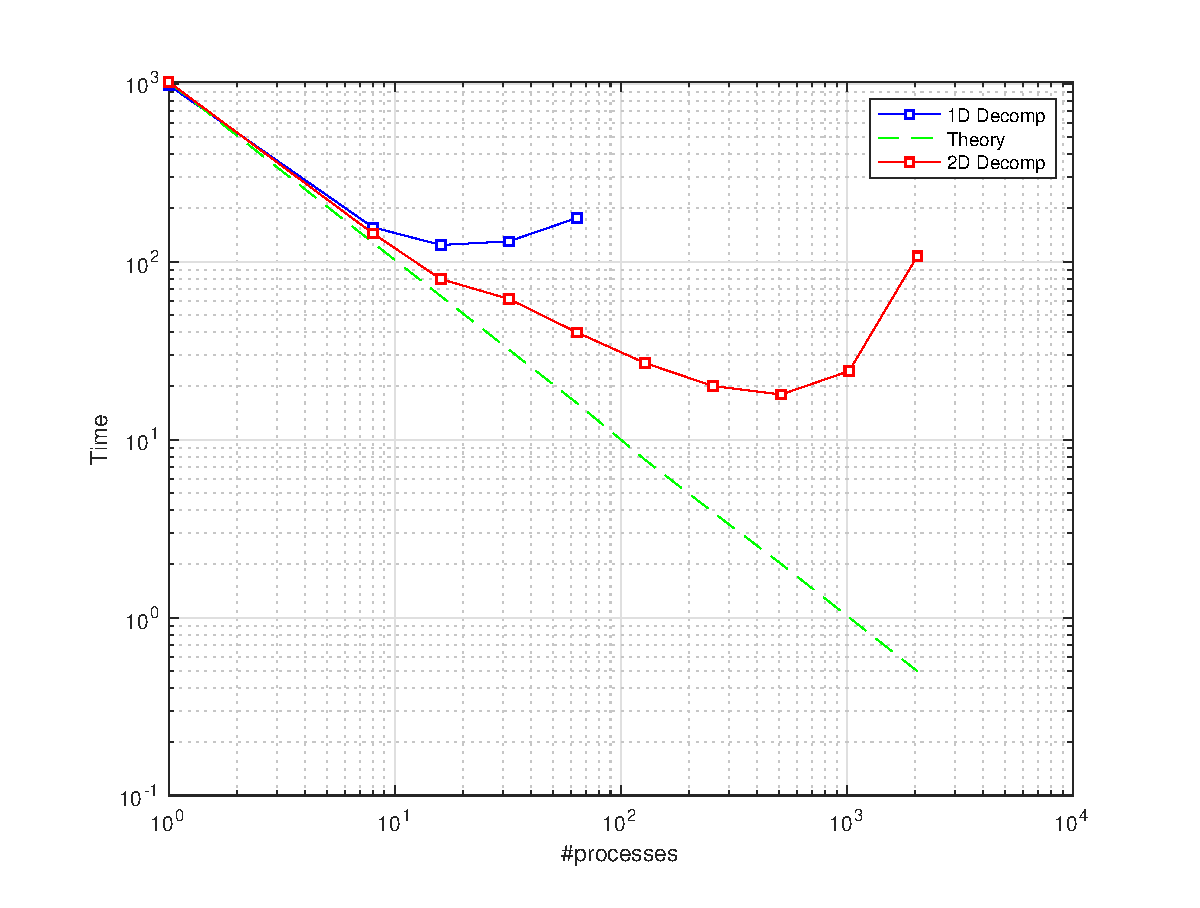
\includegraphics[scale=0.6]{grafici/641}
\caption{Scaling performance of $128^3$ simulation}
\label{641}
\end{center}
\end{figure}

In figure \ref{641} is possible to look at the time needed to perform the DNS, at varying of the cores number and algorithm.
The green dashed line represent the theoretical limit and has been obtained as the ratio between the single core time and the number of cores of the simulation.  \\
Despite of the results could seems poor, the qualitative comparison of figure~\ref{643} against a 3-dimensional FFT, using P3DFFT, reported in \cite[43]{tesi:brach}, suggest that our results are on the average, or better, until the communications cost overcome the benefits of such parallel distributed approach.

\begin{figure}
\begin{center}
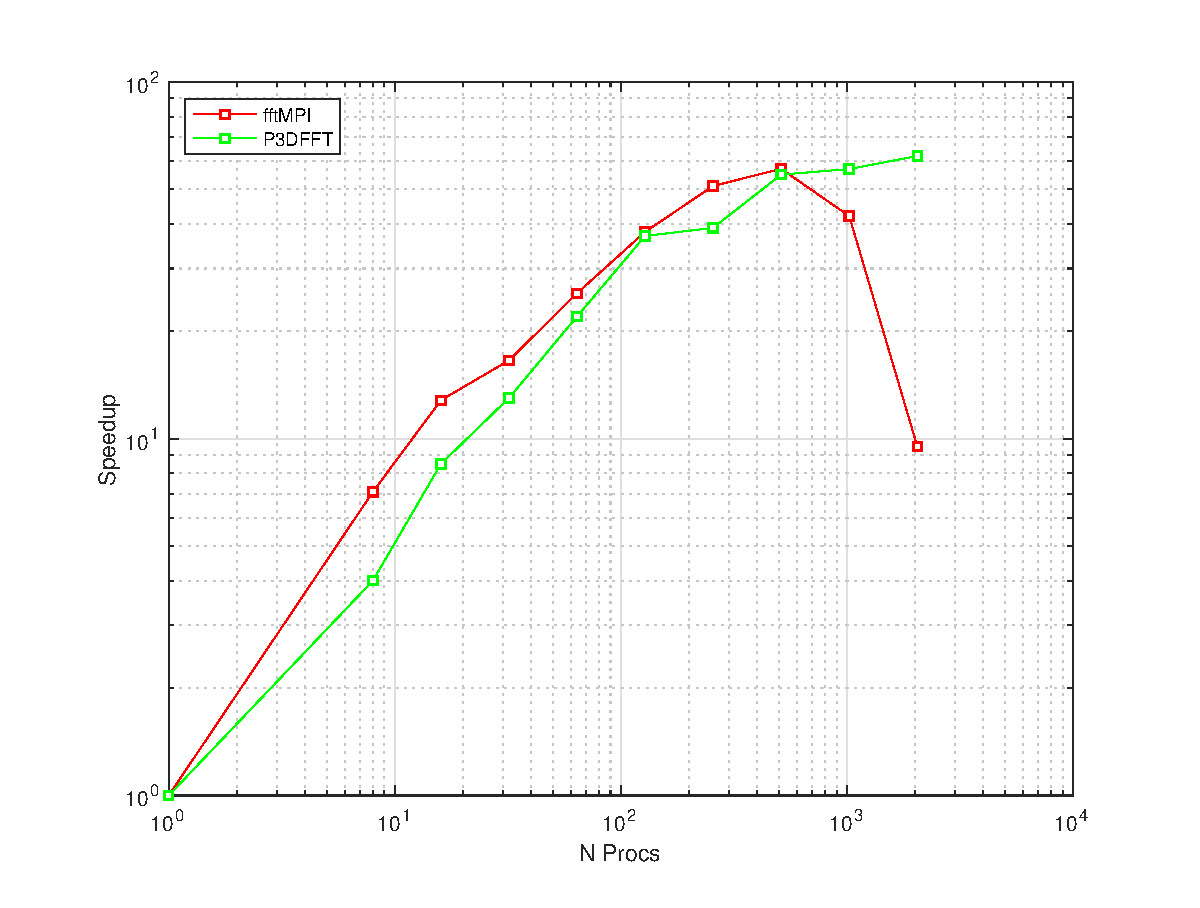
\includegraphics[scale=0.6]{grafici/643}
\caption{Comparison of a 3D FFT against DNS with fftMPI}
\label{643}
\end{center}
\end{figure}

\begin{table}[h]
\caption{Data from $128^{3}$ simulation}
\begin{center}
\begin{tabular}{c c c c c}
\toprule
\textbf{\#cores} & \textbf{Time [s]} & \textbf{Speedup} & \textbf{Efficiency [\%]} & \textbf{Decomp}\\
\midrule
\multirow{2}{*}{1} & 980 & 1.05 & 100 & 1D\\
& 1022.1 & 1 & 100 & 2D \\
\hline
\multirow{2}{*}{8} & 155.9 & 6.56 & 79 & 1D\\
& 144 & 7.1 & 89 & 2D\\
\hline
\multirow{2}{*}{16} & 124.2 & 8.24 & 49 & 1D\\
& 79.7 & 12.82 & 80 & 2D\\
\hline
\multirow{2}{*}{32} & 130.4 & 7.86 & 24 & 1D\\
& 61.7 & 16.6 & 52 & 2D\\
\hline
\multirow{2}{*}{64} & 176.1 & 5.81 & 9 & 1D\\
& 40 & 25.6 & 40 & 2D\\
\hline
128 & 26.9 & 38 & 30 & 2D\\

256 & 20 & 51.11 & 20 & 2D\\

512 & 17.9 & 57.07 & 11 & 2D\\

1024 & 24.3 & 42.1 & 4 & 2D\\

2048 & 107.3 & 9.52 & 0 & 2D\\
\bottomrule
\end{tabular}
\end{center}
\label{64data}
\end{table}%


The table~\ref{64data} on page~\pageref{64data} summarizes all data related to the $128^{3}$ simulation. 


\par
According to this table the figure \ref{642} shows the speedup at the varying of the cores number. \\
At the speedup peak the code runs $57$ times faster than serial ones. Such peak is obtained using $512$ cores. However, as expectable, the efficiency of this implementation is quite poor. In fact, if we use more than $16$ cores we drop immediately to performances around $50\%$ or lower. 
\par
Such speedup and efficiency have been calculated using the following definitions:
\[
S = \frac{T_{0}}{T_{p}} \quad \quad E = \frac{S}{p}
\]
where $T_{0}$ indicates the single core time of the pencil decomposed algorithm, $p$ is the number of cores used in the actual run, and $T_{p}$ is the time associated with it. \\
\par
For completeness the efficiency behavior is reported in figure \ref{644}.

\begin{figure}
\begin{center}
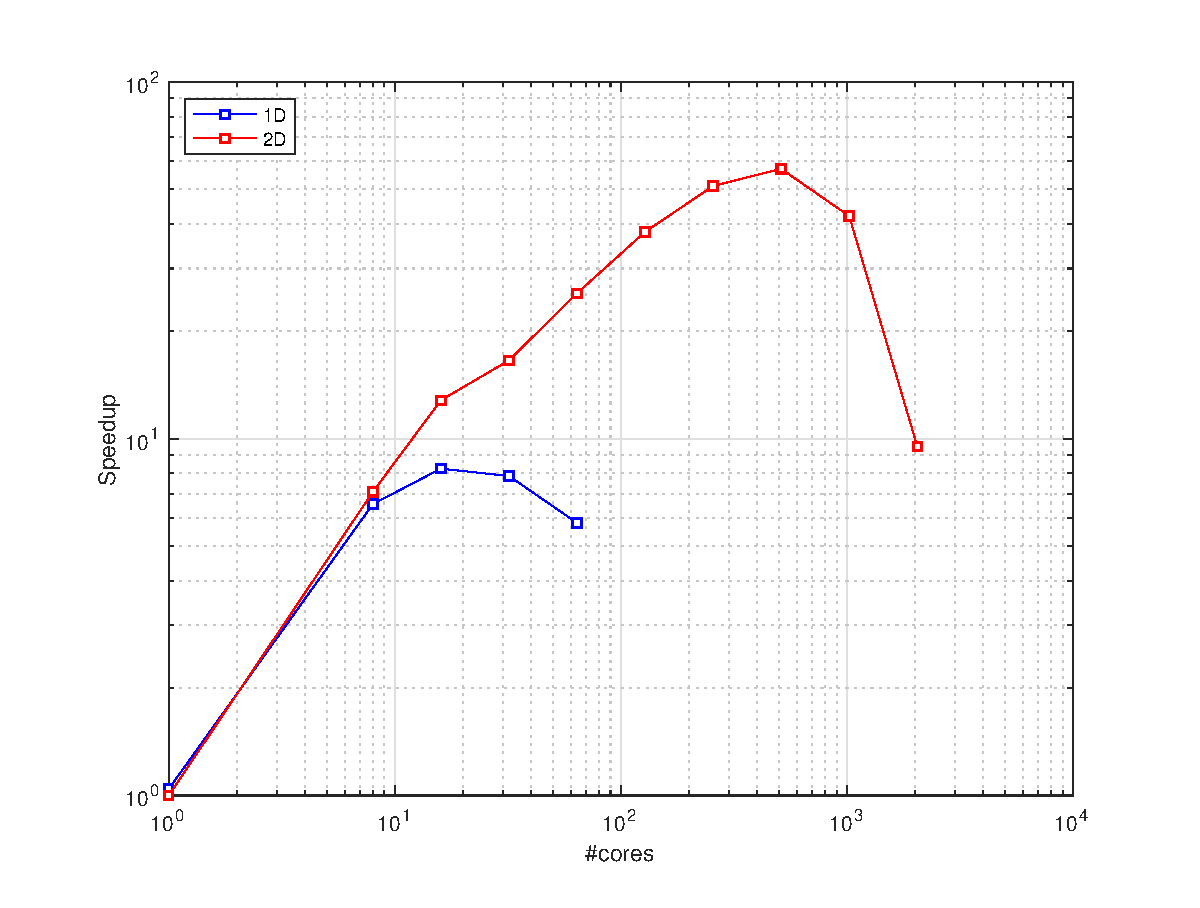
\includegraphics[scale=0.6]{grafici/642}
\caption{Speedup performance factor of $128^3$ simulation}
\label{642}
\end{center}
\end{figure}

\begin{figure}
\begin{center}
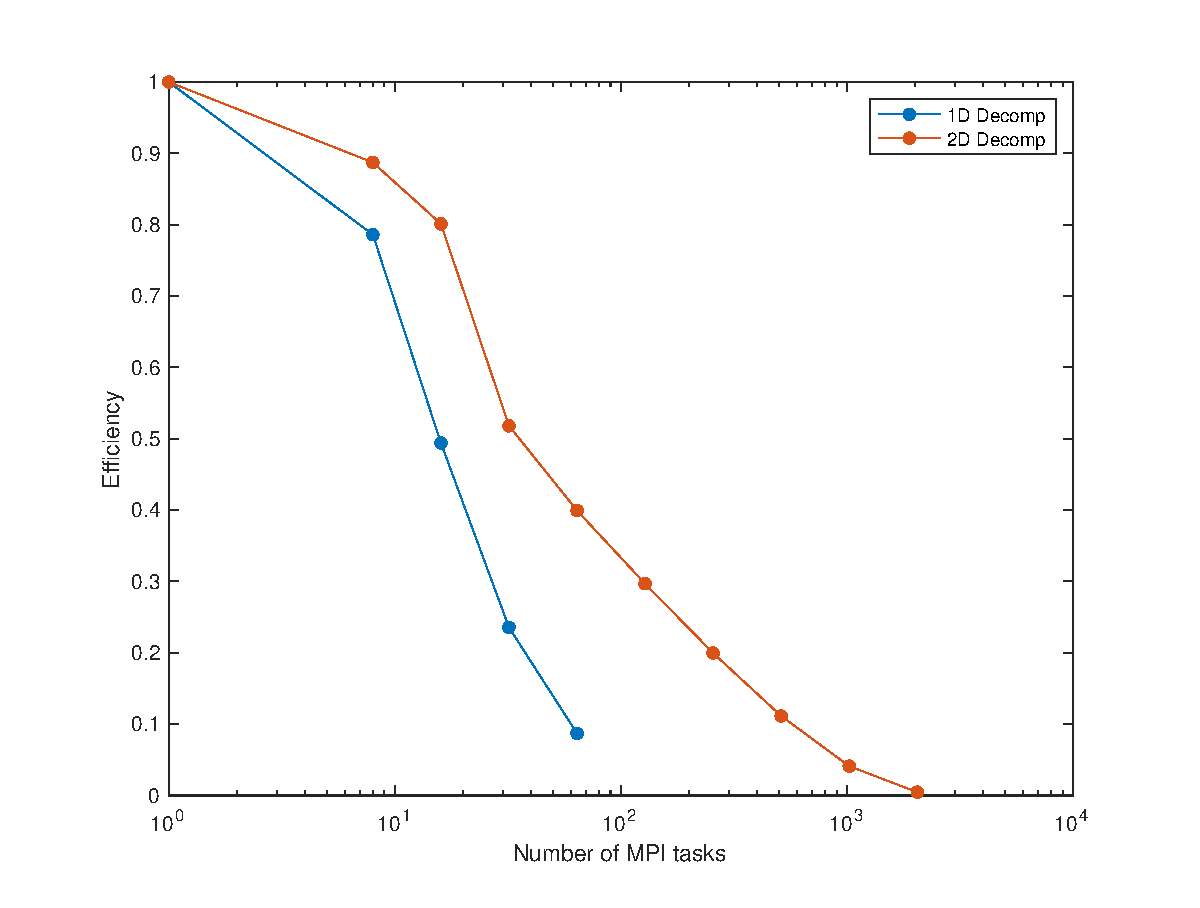
\includegraphics[scale=0.6]{grafici/644}
\caption{Efficiency factor of $128^3$ simulation}
\label{644}
\end{center}
\end{figure}
